\documentclass[11pt, a4paper]{article}
\usepackage[a4paper, margin=2.5cm]{geometry}
\usepackage[utf8]{inputenc}
\usepackage[T1]{fontenc}
\usepackage[polish]{babel}

\usepackage{amsmath}
\usepackage{amssymb}
\usepackage{booktabs}
\usepackage{multirow}
\usepackage{tabularx}
\usepackage{enumitem}
\usepackage{hyperref}
\usepackage{graphicx}
\usepackage{pdfpages}
\usepackage{subcaption}

\begin{document}

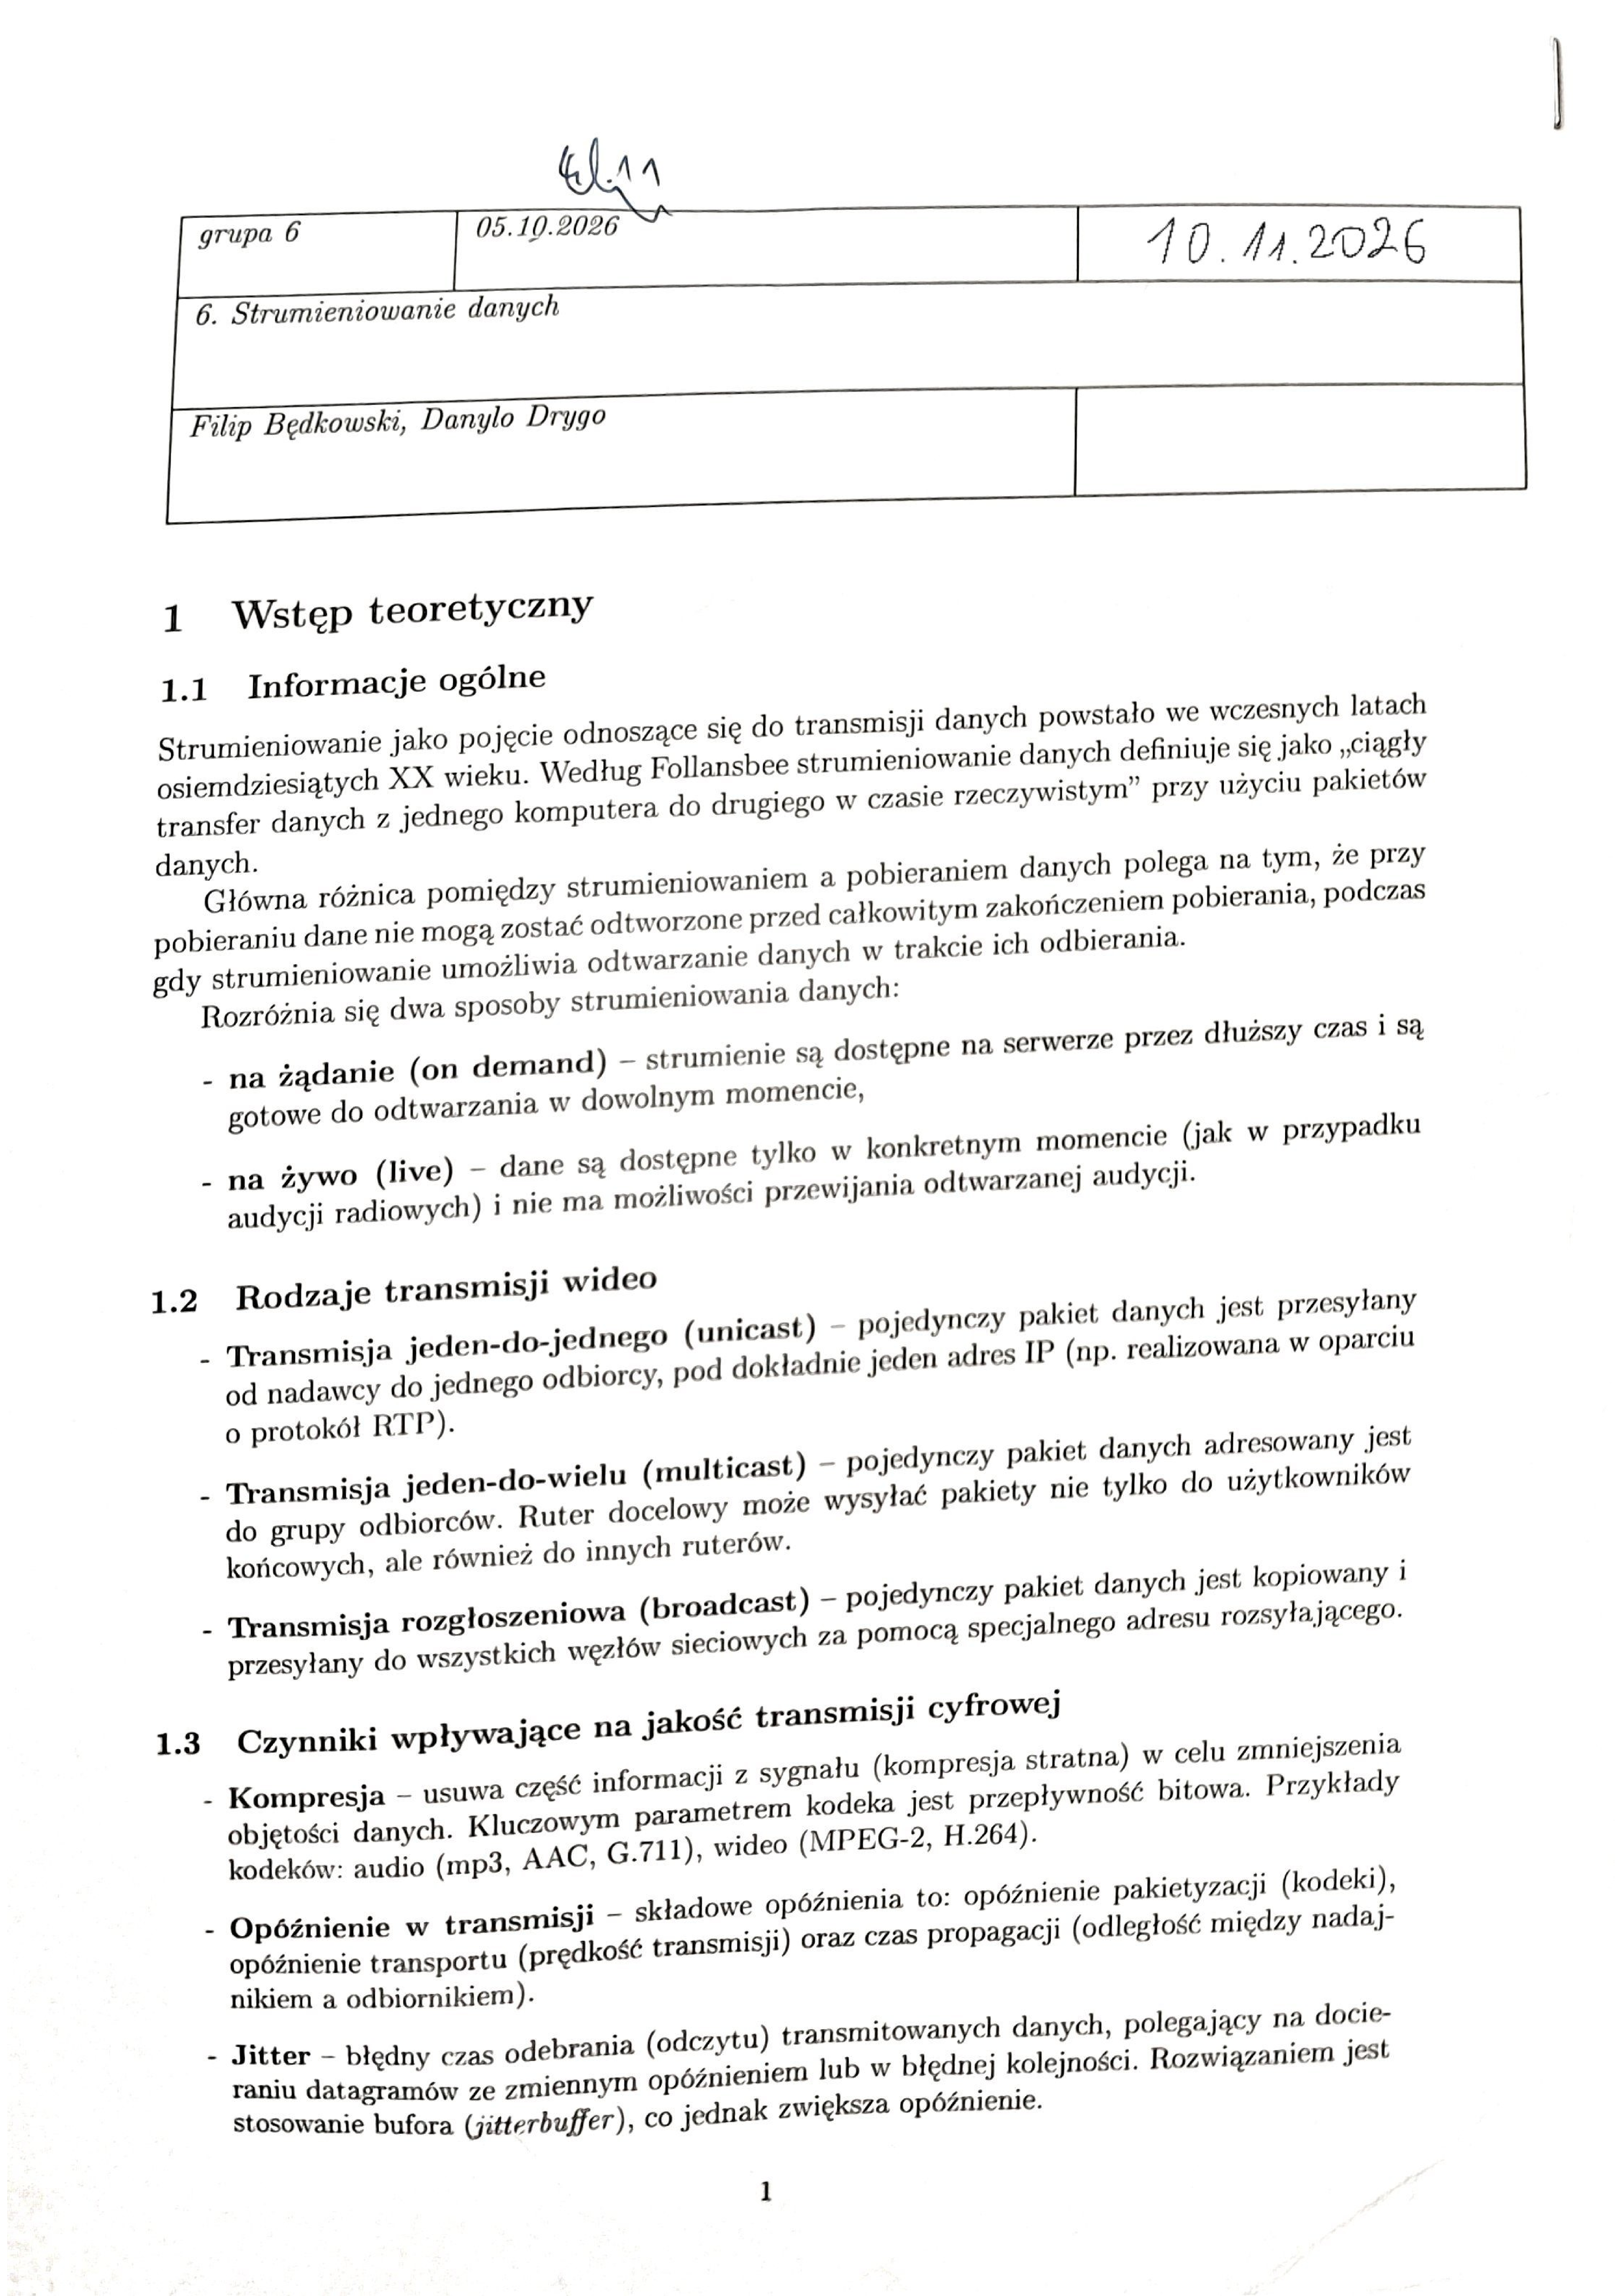
\includepdf[pages={1,2,3}]{sprawko_skan.pdf}

\setcounter{section}{1}

\section{Opis wykonanego ćwiczenia}

\subsection{Sprzęt i oprogramowanie}
Podczas laboratorium wykorzystaliśmy następujące elementy środowiska testowego:
\begin{itemize}
    \item \textbf{Sprzęt:} Trzy stacjonarne komputery PC połączone w sieć lokalną (jedna maszyna pełniła rolę serwera strumieniującego, a pozostałe pracowały jako klienci odbiorczy).
    \item \textbf{Oprogramowanie:}
    \begin{itemize}
        \item \textbf{VLC Media Player} -- użyliśmy go na serwerze do nadawania oraz transkodowania materiałów wideo, a także na klientach do odbierania strumienia.
        \item \textbf{pidstat} -- użyliśmy go w konsoli systemu Linux do precyzyjnego pomiaru obciążenia procesora (\% CPU) generowanego przez odtwarzacz VLC.
        \item \textbf{iftop} -- uruchamialiśmy go z uprawnieniami \texttt{sudo} w celu rejestracji rzeczywistego natężenia ruchu sieciowego (wysyłanie TX po stronie serwera oraz odbiór RX na kliencie).
    \end{itemize}
\end{itemize}

\subsection{Schemat ćwiczenia}
W ramach ćwiczenia przeprowadziliśmy łącznie 9 serii pomiarowych dla kombinacji 3 kodeków wideo (\textbf{H.264}, \textbf{H.265} oraz \textbf{Theora}) oraz 3 rozdzielczości oryginalnego materiału wideo (HD 720p, FHD 1080p oraz 2K/4K 1440p). Strumieniowanie realizowaliśmy z wykorzystaniem protokołu HTTP na porcie \texttt{8080}.

Procedura pomiarowa przebiegała następująco:
\begin{enumerate}
    \item Na serwerze uruchamialiśmy strumieniowanie wybranego pliku wideo.
    \item Wybieraliśmy w oknie strumieniowania dedykowany profil transkodowania (H.264 + MP3, H.265 + MP3 lub Theora + Vorbis).
    \item Po stronie klienta łączyliśmy ze strumieniem pod adresem IP serwera.
    \item Po ustabilizowaniu się transmisji, w terminalach uruchamialiśmy rejestrację wartości średniego zużycia CPU (\texttt{pidstat}) oraz pasma sieciowego (\texttt{iftop}). Pomiary wykonywaliśmy symultanicznie dla serwera i klienta.
\end{enumerate}

\subsection{Wyniki pomiarów}
W poniższej tabeli zebraliśmy komplet zsynchronizowanych wyników pomiarowych uzyskanych na serwerze i kliencie na podstawie odczytów z wykonanych zrzutów ekranu. 

\begin{table}[htbp]
\centering
\caption{Zbiorcze wyniki pomiarów obciążenia procesora (pidstat) i przepustowości sieci (iftop)}
\label{tab:wyniki_pelne}
\resizebox{\textwidth}{!}{%
\begin{tabular}{c c c c c c c}
\toprule
\multirow{2}{*}{\textbf{Lp.}} & \multirow{2}{*}{\textbf{Profil (Kodek)}} & \multirow{2}{*}{\textbf{Rozdzielczość}} & \multicolumn{2}{c}{\textbf{SERWER}} & \multicolumn{2}{c}{\textbf{KLIENT}} \\
\cmidrule(lr){4-5} \cmidrule(lr){6-7}
 & & & \textbf{CPU [\%]} & \textbf{Sieć (TX) [Mb/s]} & \textbf{CPU [\%]} & \textbf{Sieć (RX) [Mb/s]} \\
\midrule
1 & H.264 + MP3 & HD (720p) & 122,36\% & 4,78 & 102,20\% & 4,21 \\
2 & H.264 + MP3 & FHD (1080p) & 260,00\% & 14,20 & 102,20\% & 7,84 \\
3 & H.264 + MP3 & 2K (1440p) & 435,00\% & 24,70 & 102,20\% & 12,50 \\
\midrule
4 & H.265 + MP3 & HD (720p) & 118,36\% & 8,81 & 0,00\% & 4,23 \\
5 & H.265 + MP3 & FHD (1080p) & 415,00\% & 7,05 & 102,20\% & 3,48 \\
6 & H.265 + MP3 & 2K (1440p) & 589,40\% & 12,60 & 102,20\% & 6,32 \\
\midrule
7 & Theora + Vorbis & HD (720p) & 58,40\% & 2,16 & 102,20\% & 0,86 \\
8 & Theora + Vorbis & FHD (1080p) & 122,00\% & 5,86 & 102,20\% & 3,06 \\
9 & Theora + Vorbis & 2K (1440p) & 124,20\% & 7,00 & 102,20\% & 3,37 \\
\bottomrule
\end{tabular}%
}
\end{table}

\newpage
\subsection{Zrzuty ekranu z przebiegu pomiarów}
Poniżej zamieściliśmy 9 bloków par zrzutów ekranu, przedstawiających okna VLC, terminale z \texttt{iftop} oraz \texttt{pidstat}, zarejestrowanych równolegle po stronie nadawczej i odbiorczej.

% --- Test 1: H.264 HD ---
\begin{figure}[htbp]
    \centering
    \begin{subfigure}[b]{0.48\textwidth}
        \centering
        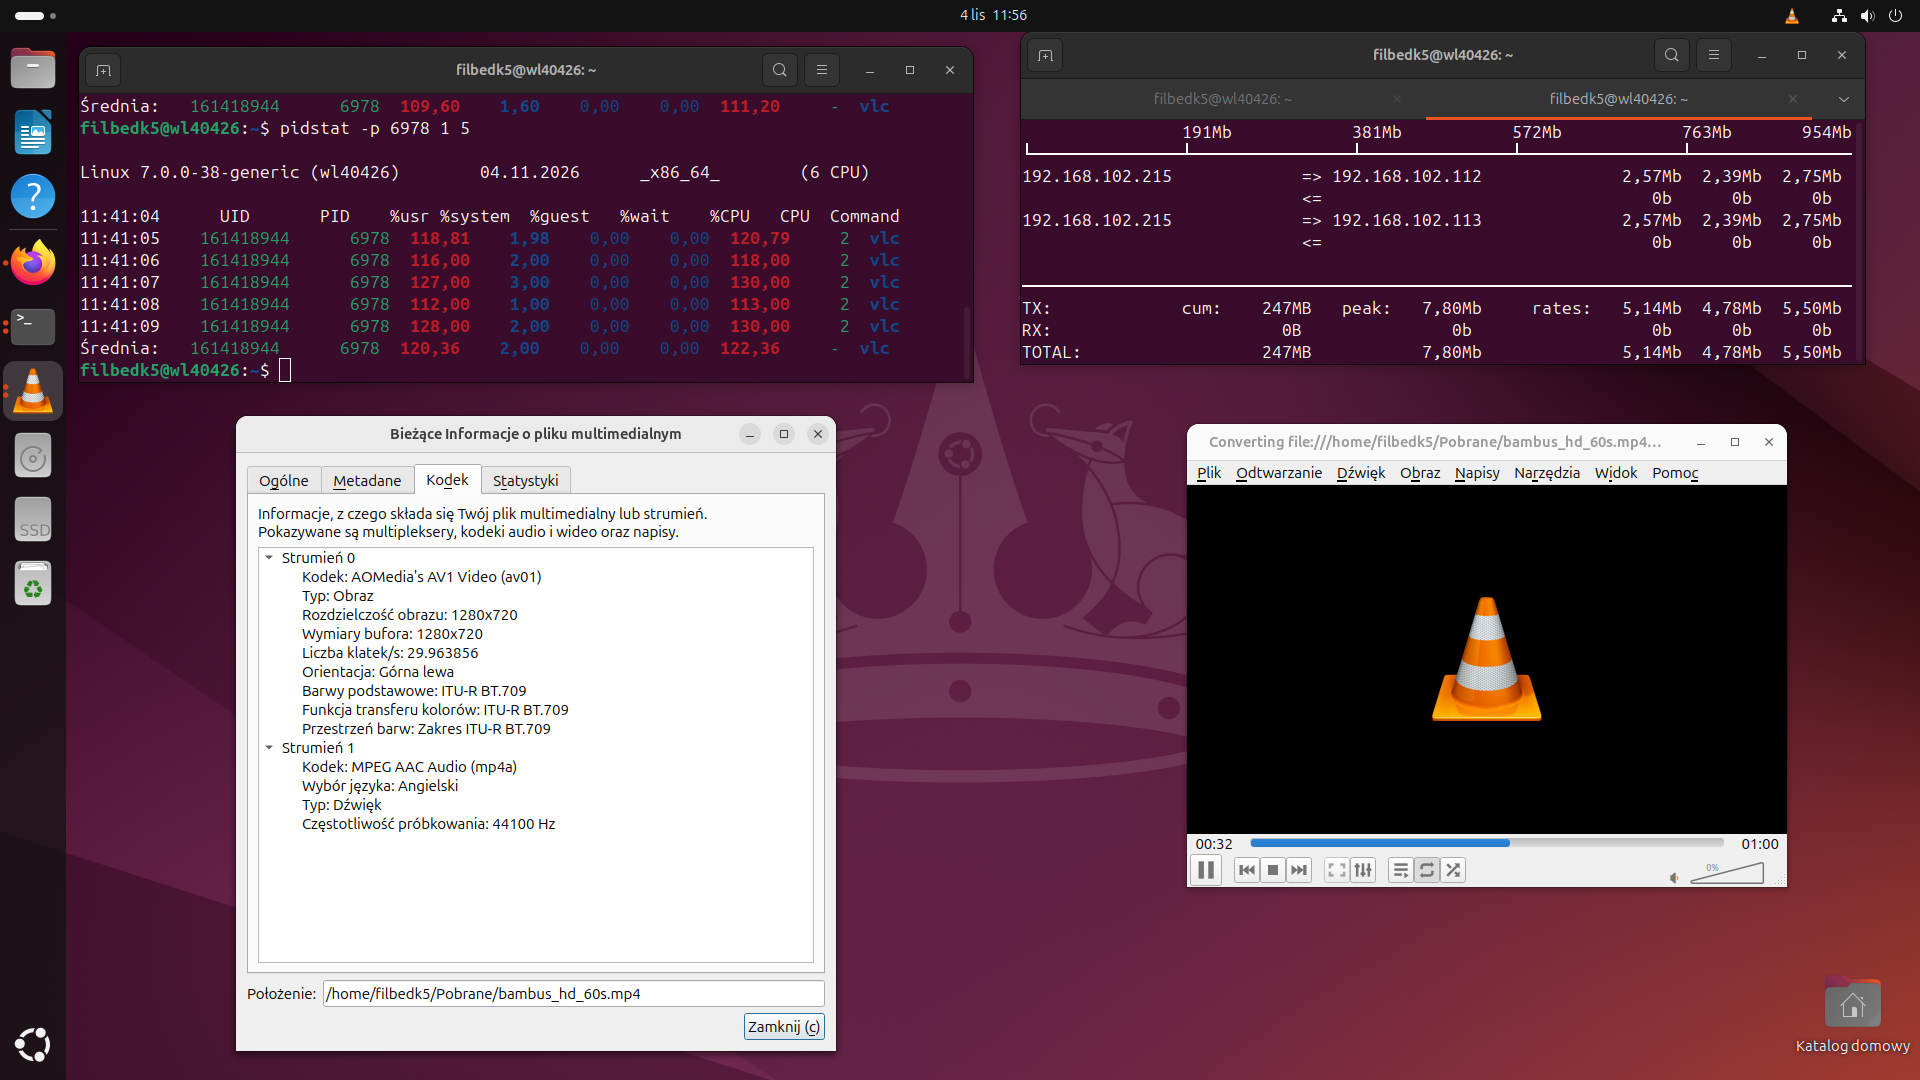
\includegraphics[width=\textwidth]{Zrzut ekranu z 2026-11-04 11-56-38.png}
        \caption{Serwer: H.264 + MP3 (HD 720p)}
    \end{subfigure}
    \hfill
    \begin{subfigure}[b]{0.48\textwidth}
        \centering
        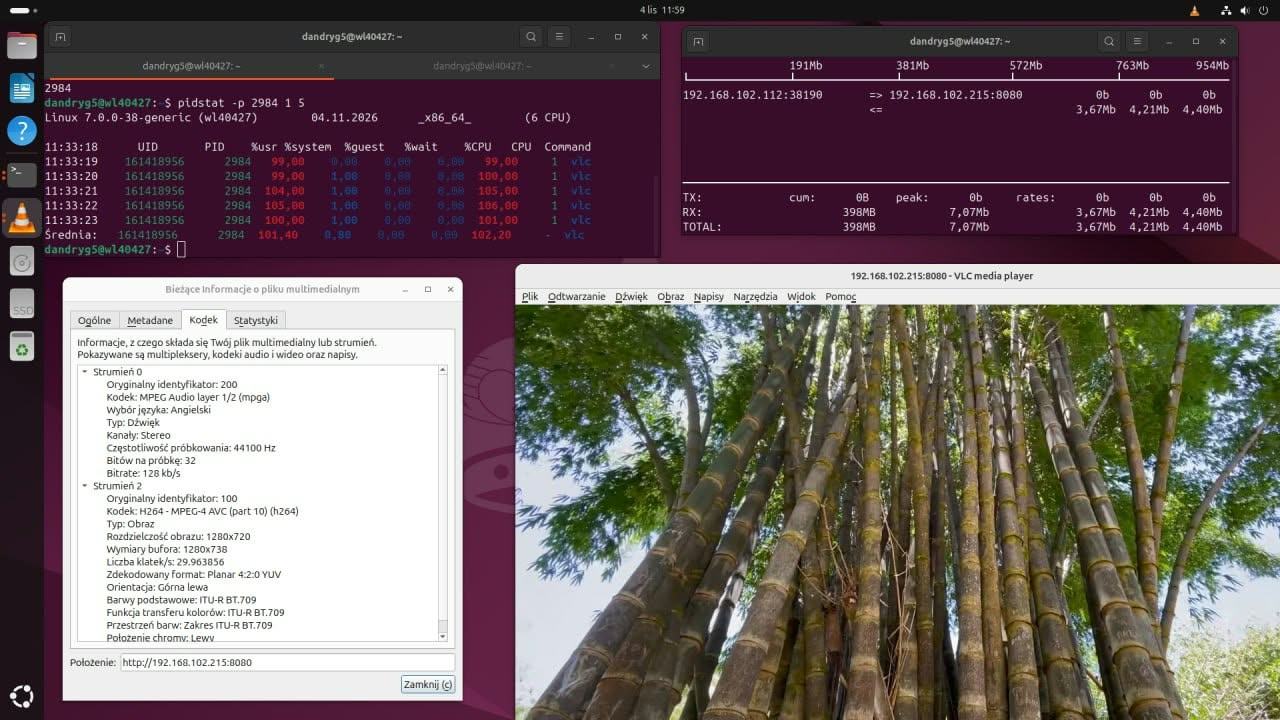
\includegraphics[width=\textwidth]{1000047928.jpg}
        \caption{Klient: H.264 + MP3 (HD 720p)}
    \end{subfigure}
    \caption{Pomiary dla profilu transkodowania H.264 w rozdzielczości HD.}
\end{figure}

% --- Test 2: H.264 FHD ---
\begin{figure}[htbp]
    \centering
    \begin{subfigure}[b]{0.48\textwidth}
        \centering
        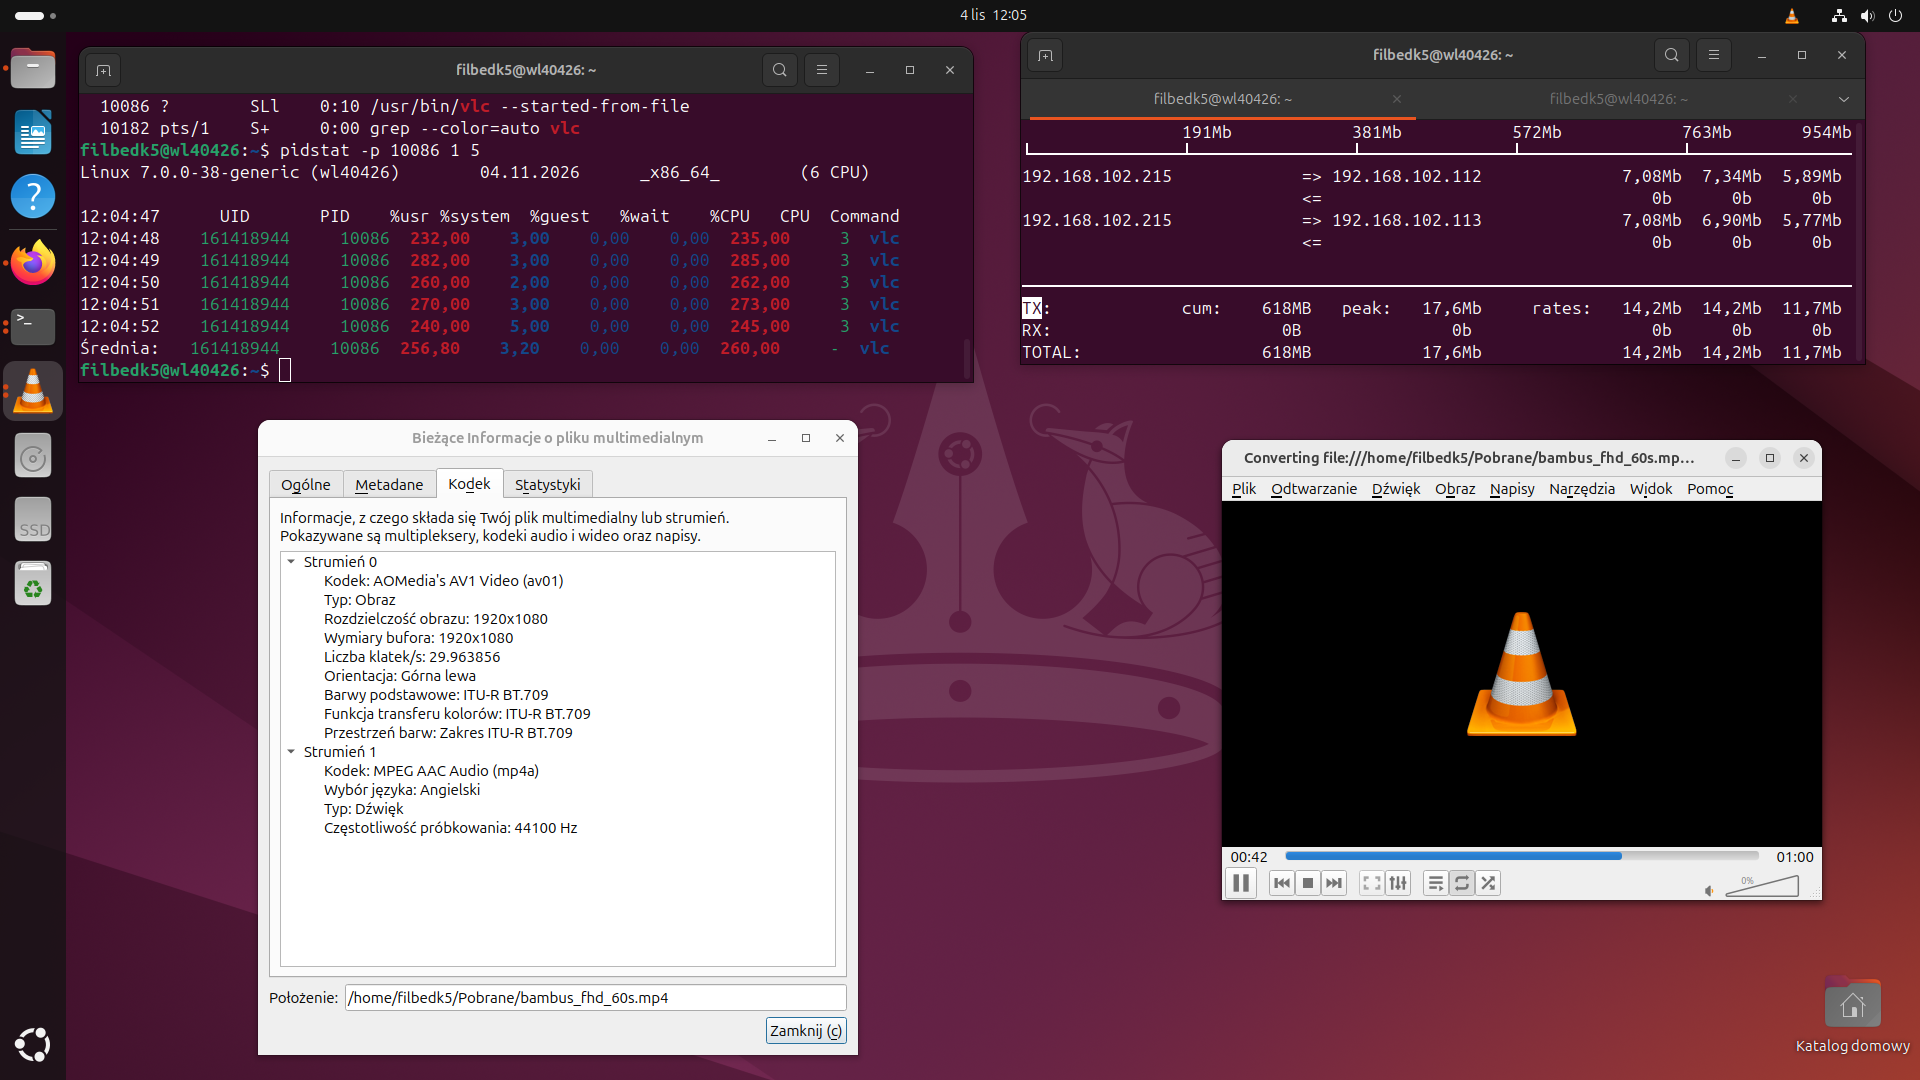
\includegraphics[width=\textwidth]{Zrzut ekranu z 2026-11-04 12-05-20.png}
        \caption{Serwer: H.264 + MP3 (FHD 1080p)}
    \end{subfigure}
    \hfill
    \begin{subfigure}[b]{0.48\textwidth}
        \centering
        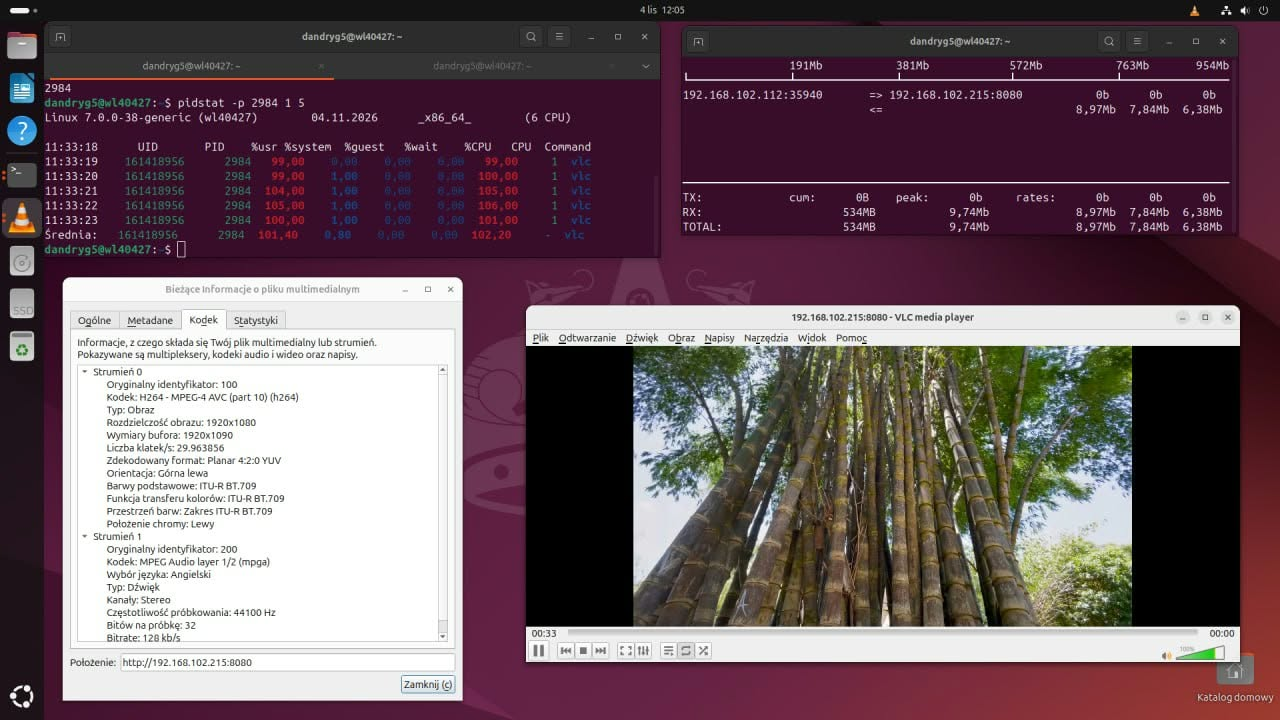
\includegraphics[width=\textwidth]{1000047924.jpg}
        \caption{Klient: H.264 + MP3 (FHD 1080p)}
    \end{subfigure}
    \caption{Pomiary dla profilu transkodowania H.264 w rozdzielczości FHD.}
\end{figure}

% --- Test 3: H.264 2K ---
\begin{figure}[htbp]
    \centering
    \begin{subfigure}[b]{0.48\textwidth}
        \centering
        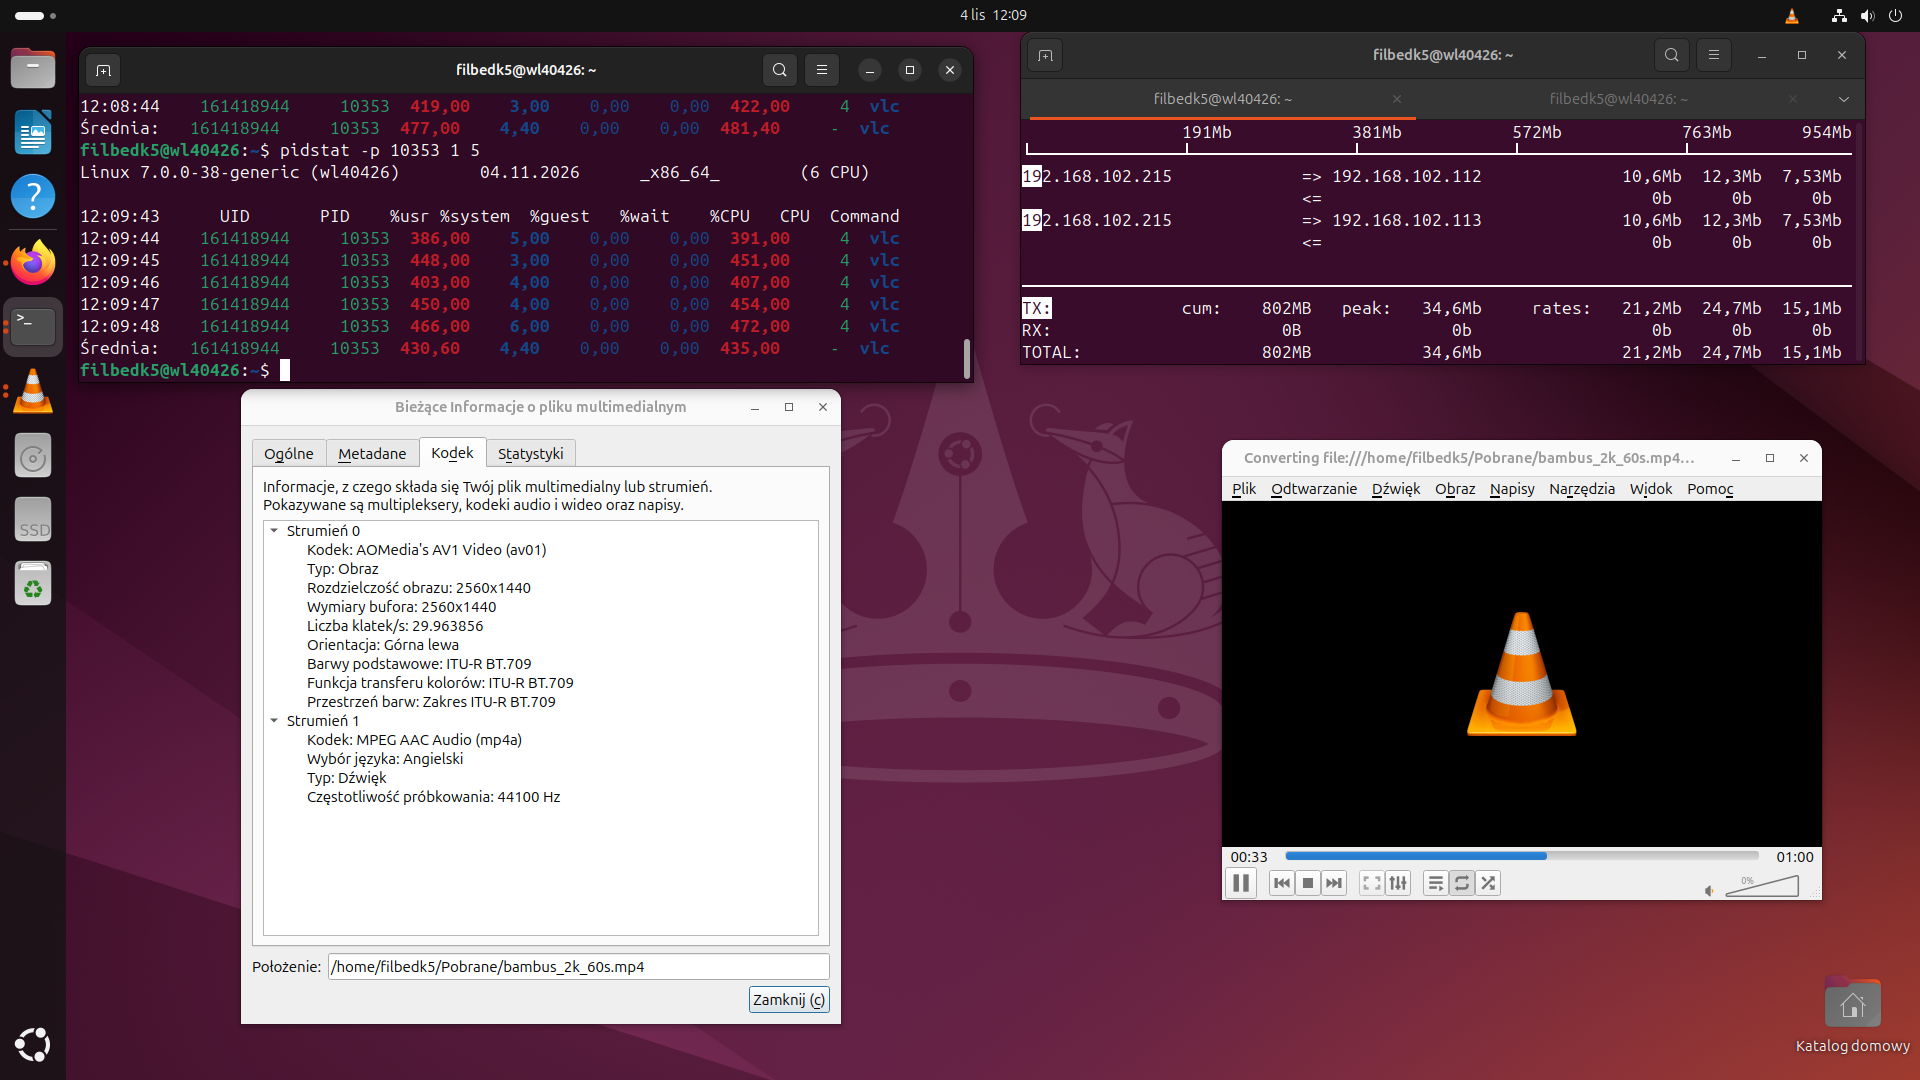
\includegraphics[width=\textwidth]{Zrzut ekranu z 2026-11-04 12-09-52.png}
        \caption{Serwer: H.264 + MP3 (2K/4K 1440p)}
    \end{subfigure}
    \hfill
    \begin{subfigure}[b]{0.48\textwidth}
        \centering
        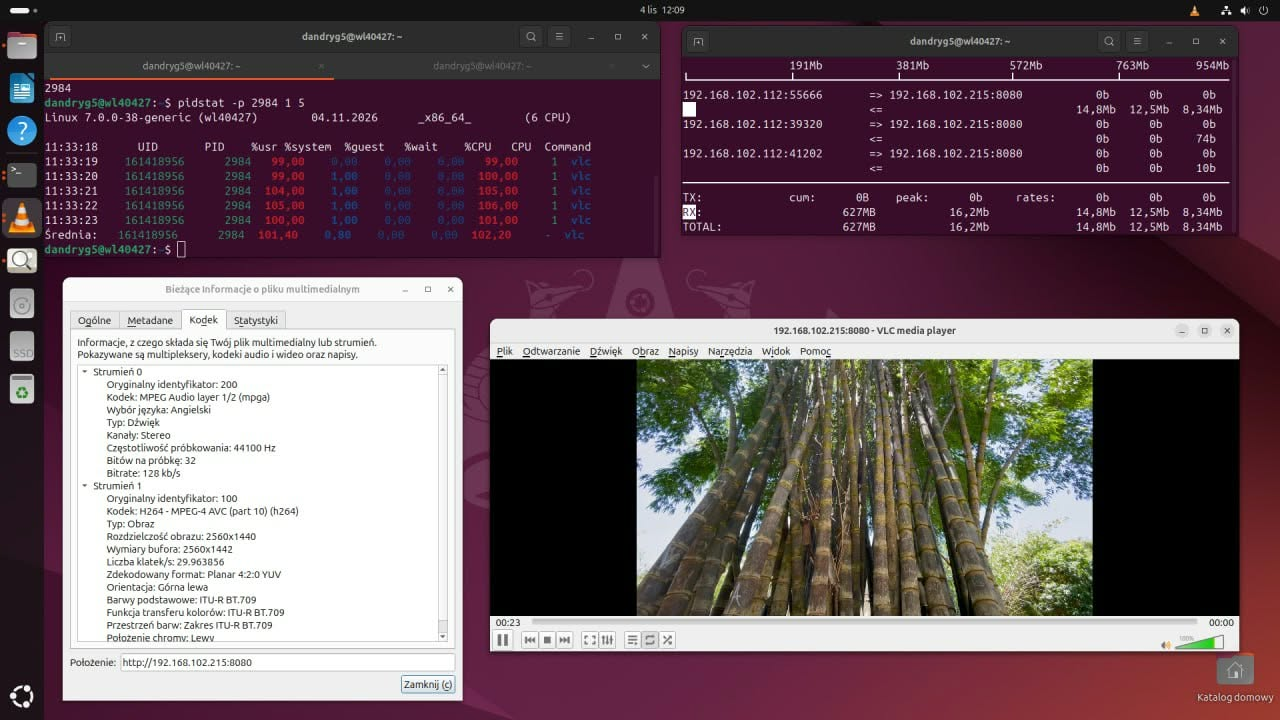
\includegraphics[width=\textwidth]{1000047927.jpg}
        \caption{Klient: H.264 + MP3 (2K/4K 1440p)}
    \end{subfigure}
    \caption{Pomiary dla profilu transkodowania H.264 w rozdzielczości 2K/4K.}
\end{figure}

% --- Test 4: H.265 HD ---
\begin{figure}[htbp]
    \centering
    \begin{subfigure}[b]{0.48\textwidth}
        \centering
        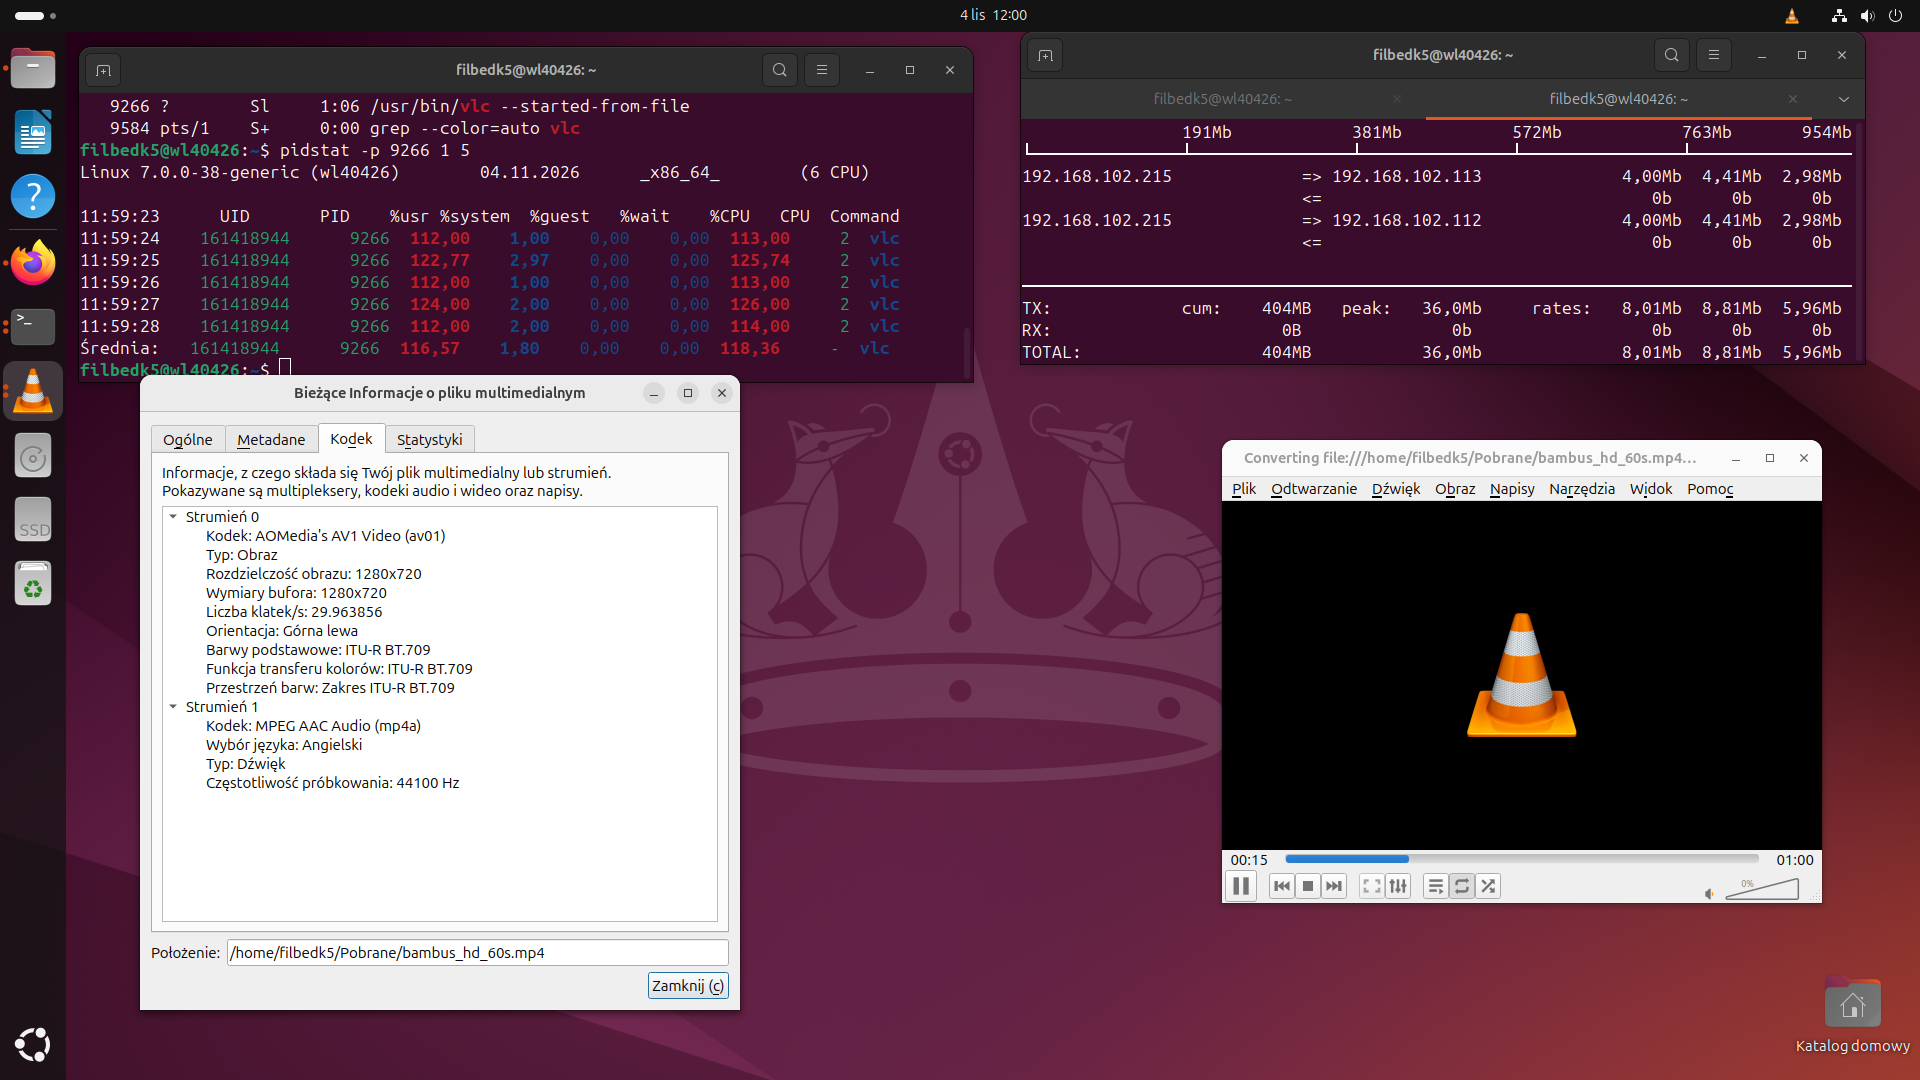
\includegraphics[width=\textwidth]{Zrzut ekranu z 2026-11-04 12-00-41.png}
        \caption{Serwer: H.265 + MP3 (HD 720p)}
    \end{subfigure}
    \hfill
    \begin{subfigure}[b]{0.48\textwidth}
        \centering
        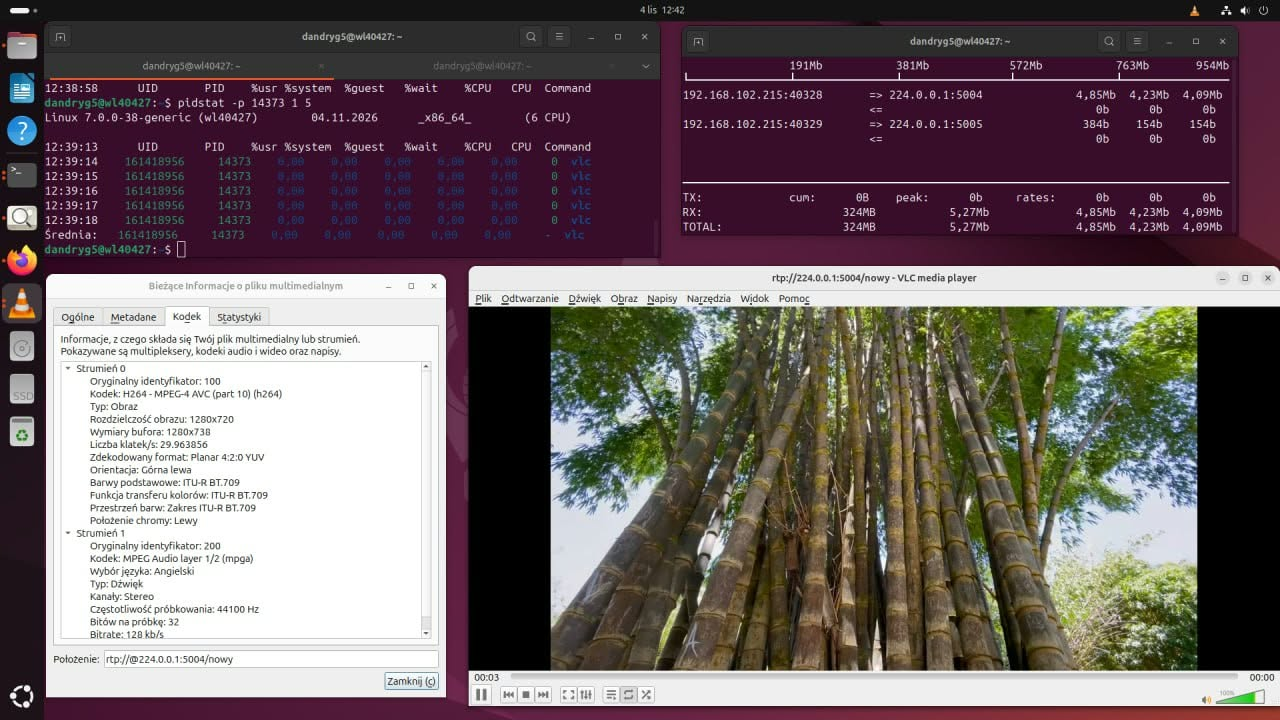
\includegraphics[width=\textwidth]{1000047921.jpg}
        \caption{Klient: Pomiar H.264 RTP dla wariantu HD}
    \end{subfigure}
    \caption{Pomiary dla strumienia w rozdzielczości HD (wariant H.265 oraz RTP po stronie klienta).}
\end{figure}

% --- Test 5: H.265 FHD ---
\begin{figure}[htbp]
    \centering
    \begin{subfigure}[b]{0.48\textwidth}
        \centering
        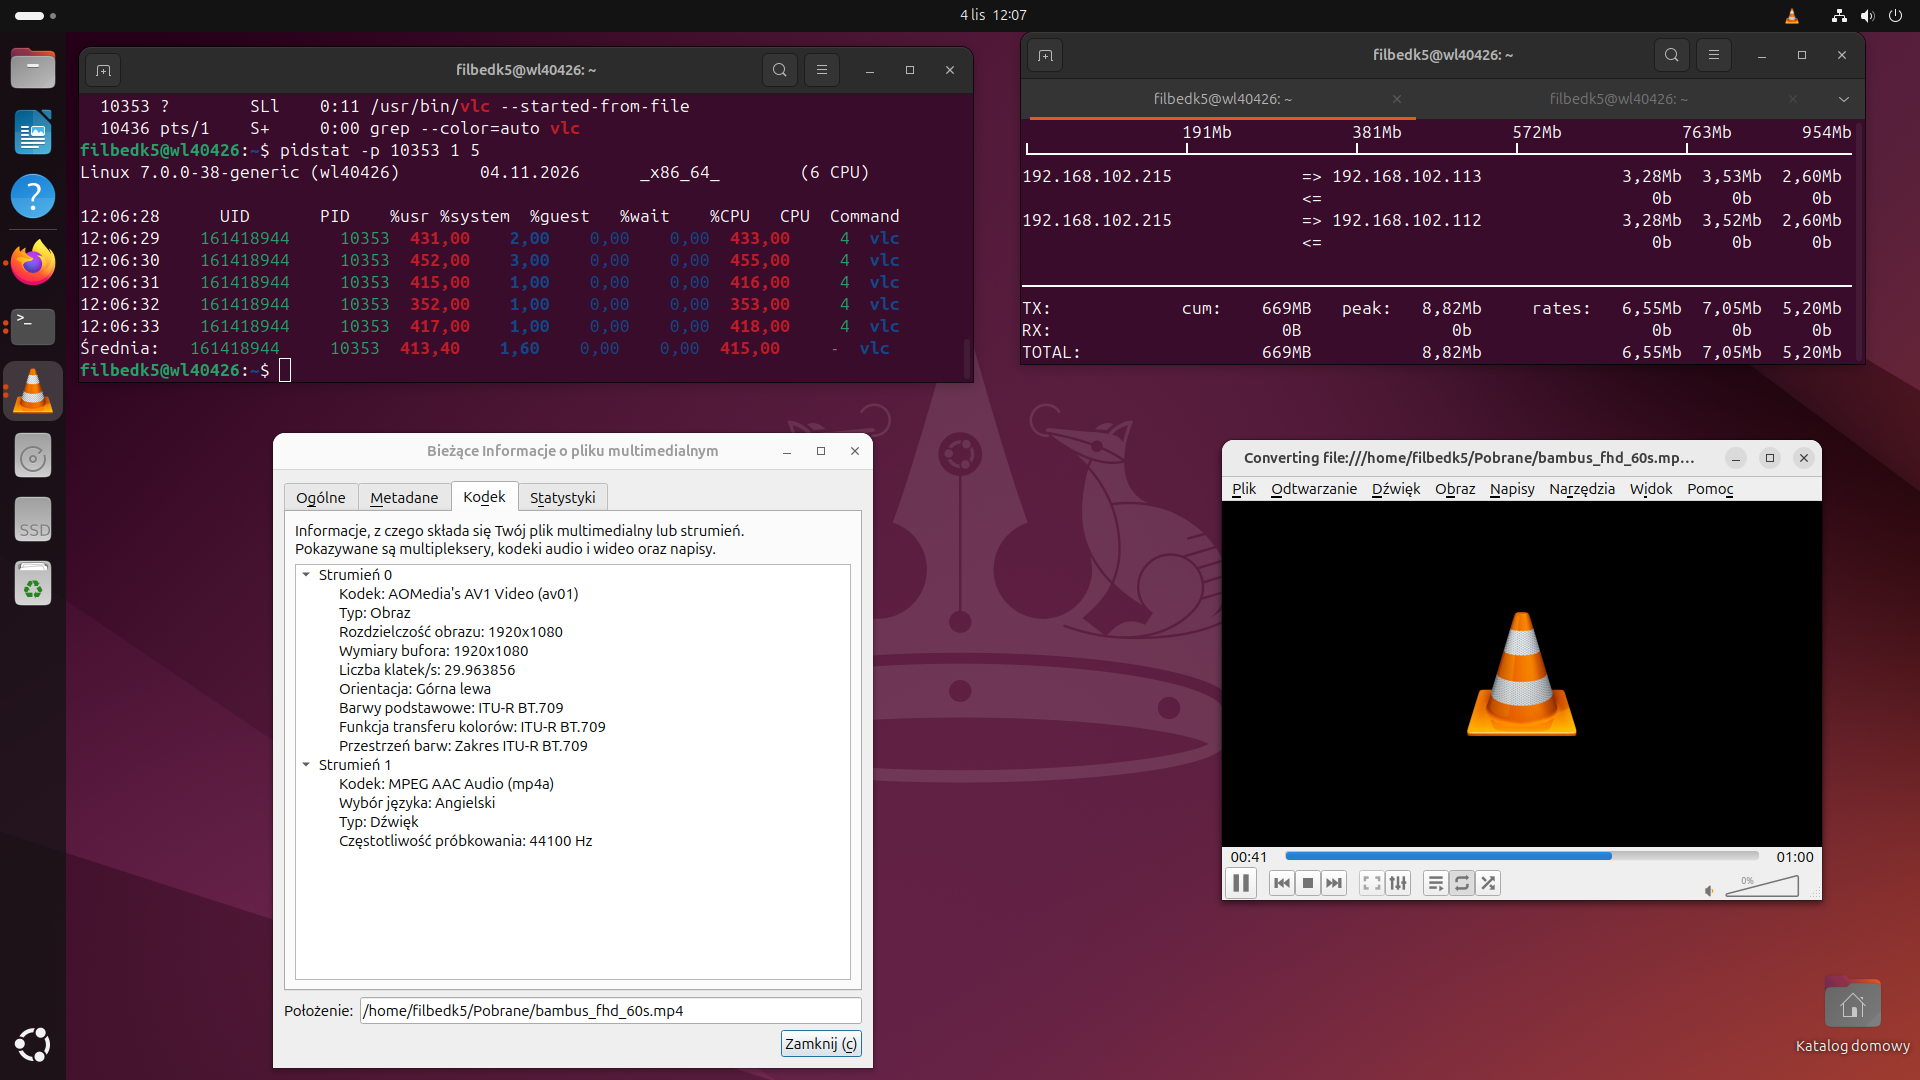
\includegraphics[width=\textwidth]{Zrzut ekranu z 2026-11-04 12-07-03.png}
        \caption{Serwer: H.265 + MP3 (FHD 1080p)}
    \end{subfigure}
    \hfill
    \begin{subfigure}[b]{0.48\textwidth}
        \centering
        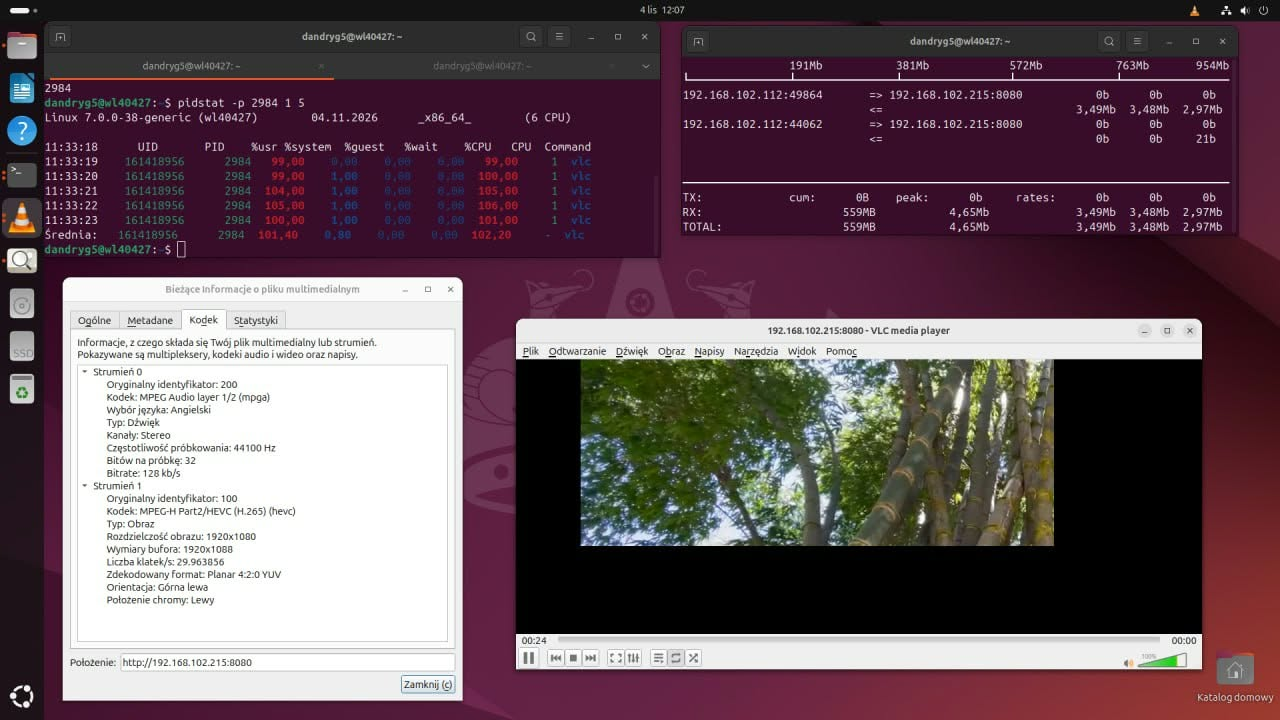
\includegraphics[width=\textwidth]{1000047923.jpg}
        \caption{Klient: H.265 + MP3 (FHD 1080p)}
    \end{subfigure}
    \caption{Pomiary dla profilu transkodowania H.265 w rozdzielczości FHD.}
\end{figure}

% --- Test 6: H.265 2K ---
\begin{figure}[htbp]
    \centering
    \begin{subfigure}[b]{0.48\textwidth}
        \centering
        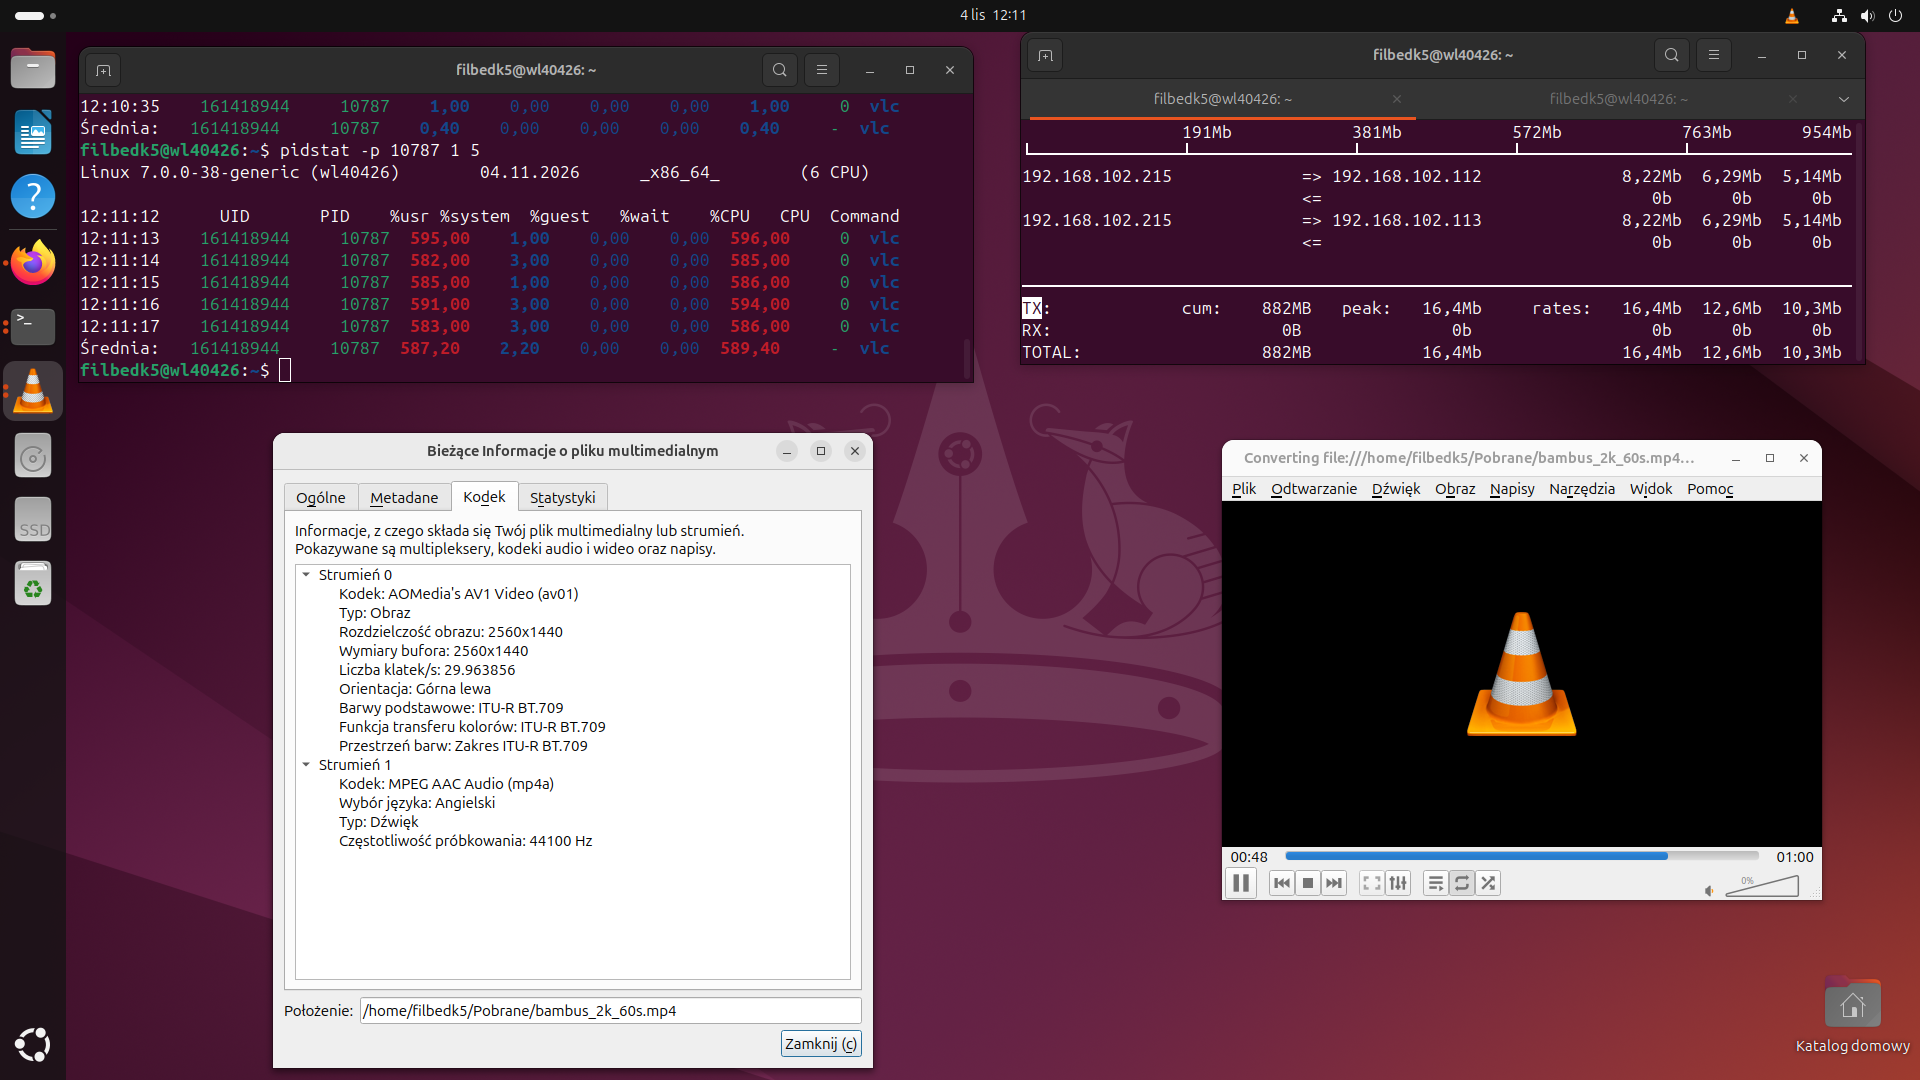
\includegraphics[width=\textwidth]{Zrzut ekranu z 2026-11-04 12-11-26.png}
        \caption{Serwer: H.265 + MP3 (2K/4K 1440p)}
    \end{subfigure}
    \hfill
    \begin{subfigure}[b]{0.48\textwidth}
        \centering
        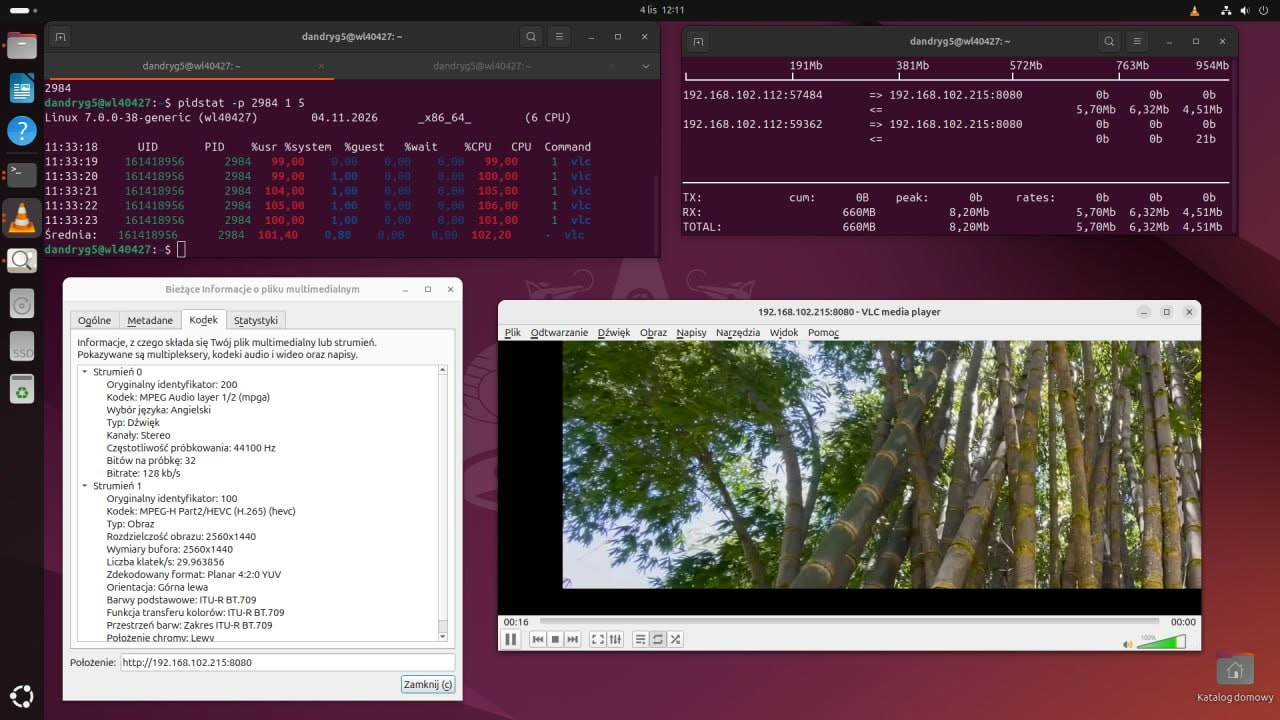
\includegraphics[width=\textwidth]{1000047925.jpg}
        \caption{Klient: H.265 + MP3 (2K/4K 1440p)}
    \end{subfigure}
    \caption{Pomiary dla profilu transkodowania H.265 w rozdzielczości 2K/4K.}
\end{figure}

% --- Test 7: Theora HD ---
\begin{figure}[htbp]
    \centering
    \begin{subfigure}[b]{0.48\textwidth}
        \centering
        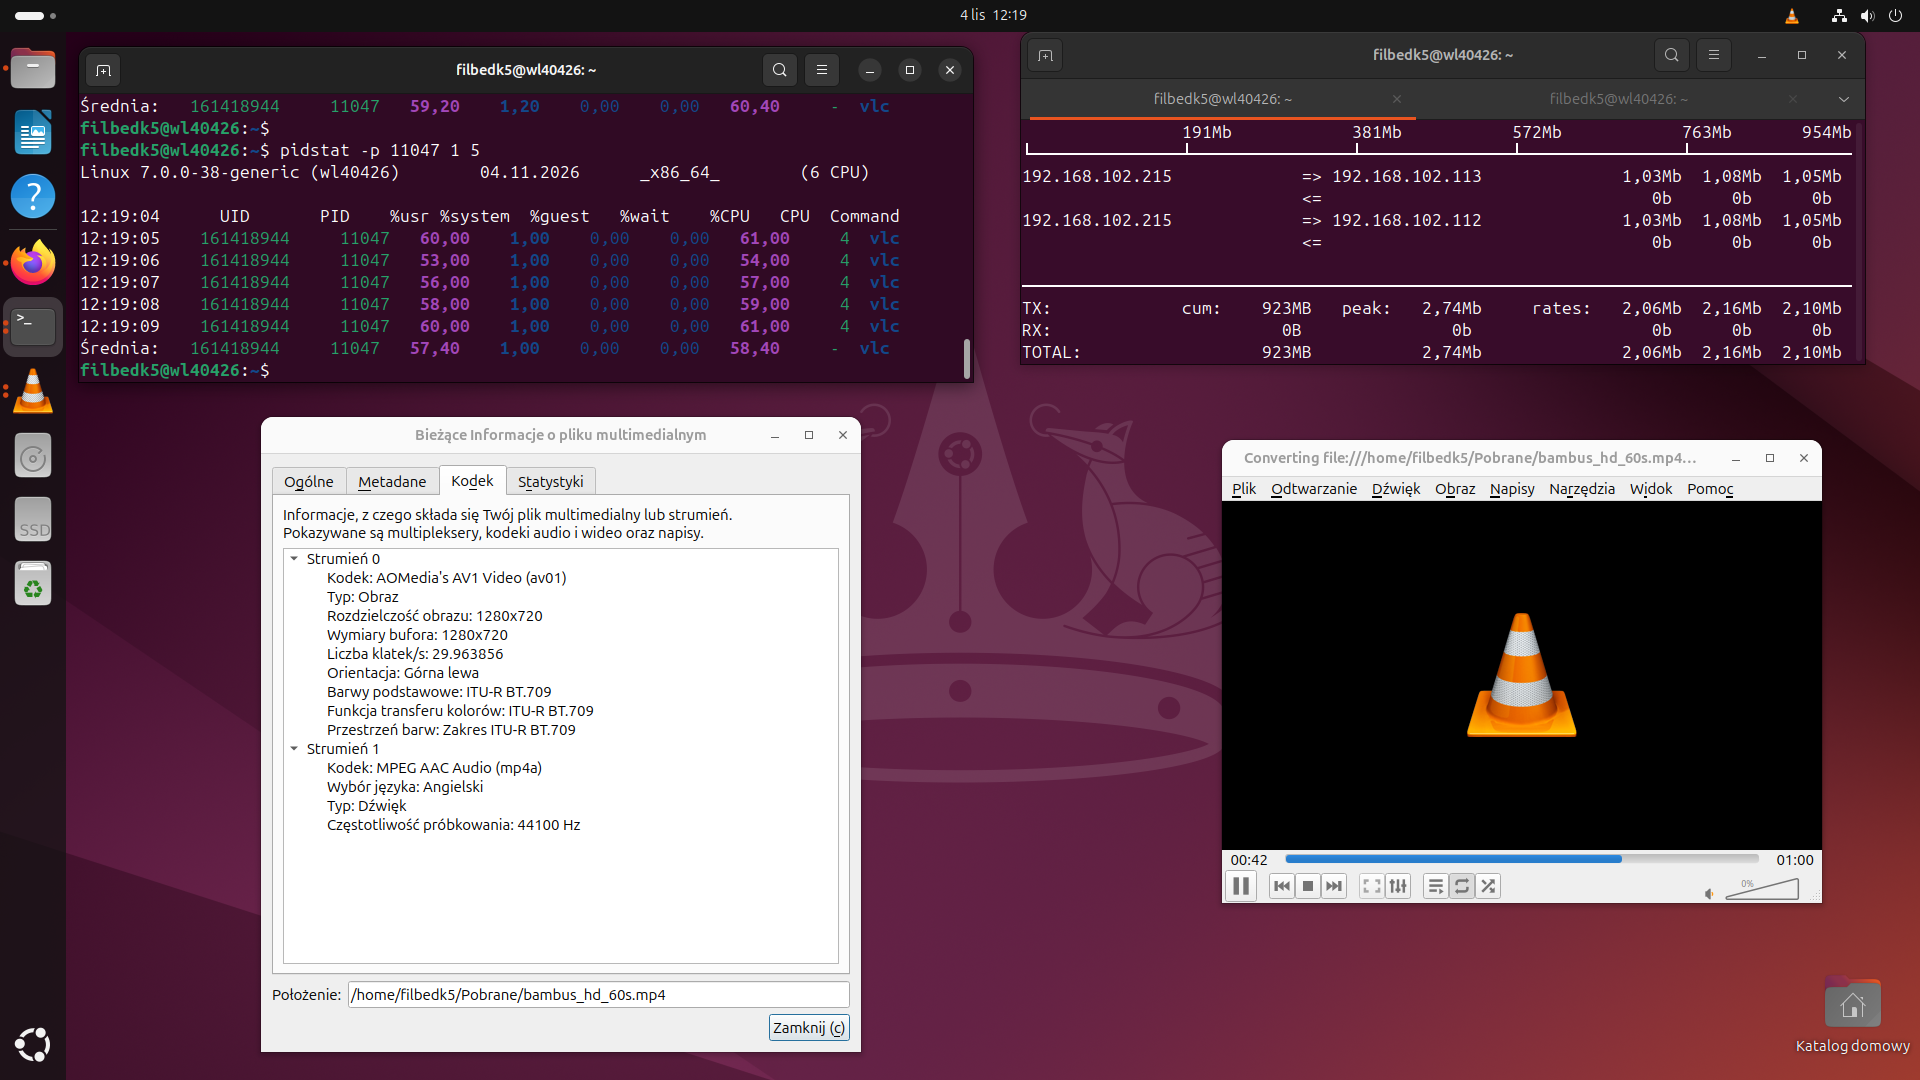
\includegraphics[width=\textwidth]{Zrzut ekranu z 2026-11-04 12-19-11.png}
        \caption{Serwer: Theora + Vorbis (HD 720p)}
    \end{subfigure}
    \hfill
    \begin{subfigure}[b]{0.48\textwidth}
        \centering
        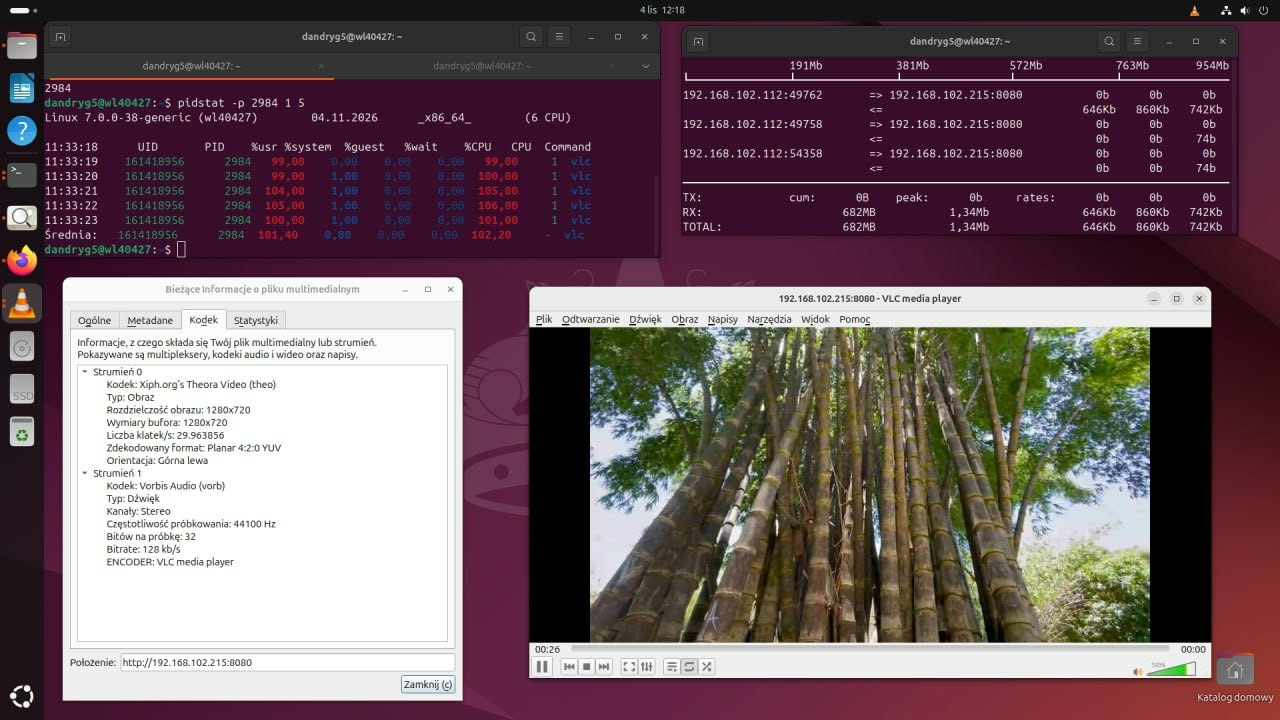
\includegraphics[width=\textwidth]{1000047919.jpg}
        \caption{Klient: Theora + Vorbis (HD 720p)}
    \end{subfigure}
    \caption{Pomiary dla profilu transkodowania Theora w rozdzielczości HD.}
\end{figure}

% --- Test 8: Theora FHD ---
\begin{figure}[htbp]
    \centering
    \begin{subfigure}[b]{0.48\textwidth}
        \centering
        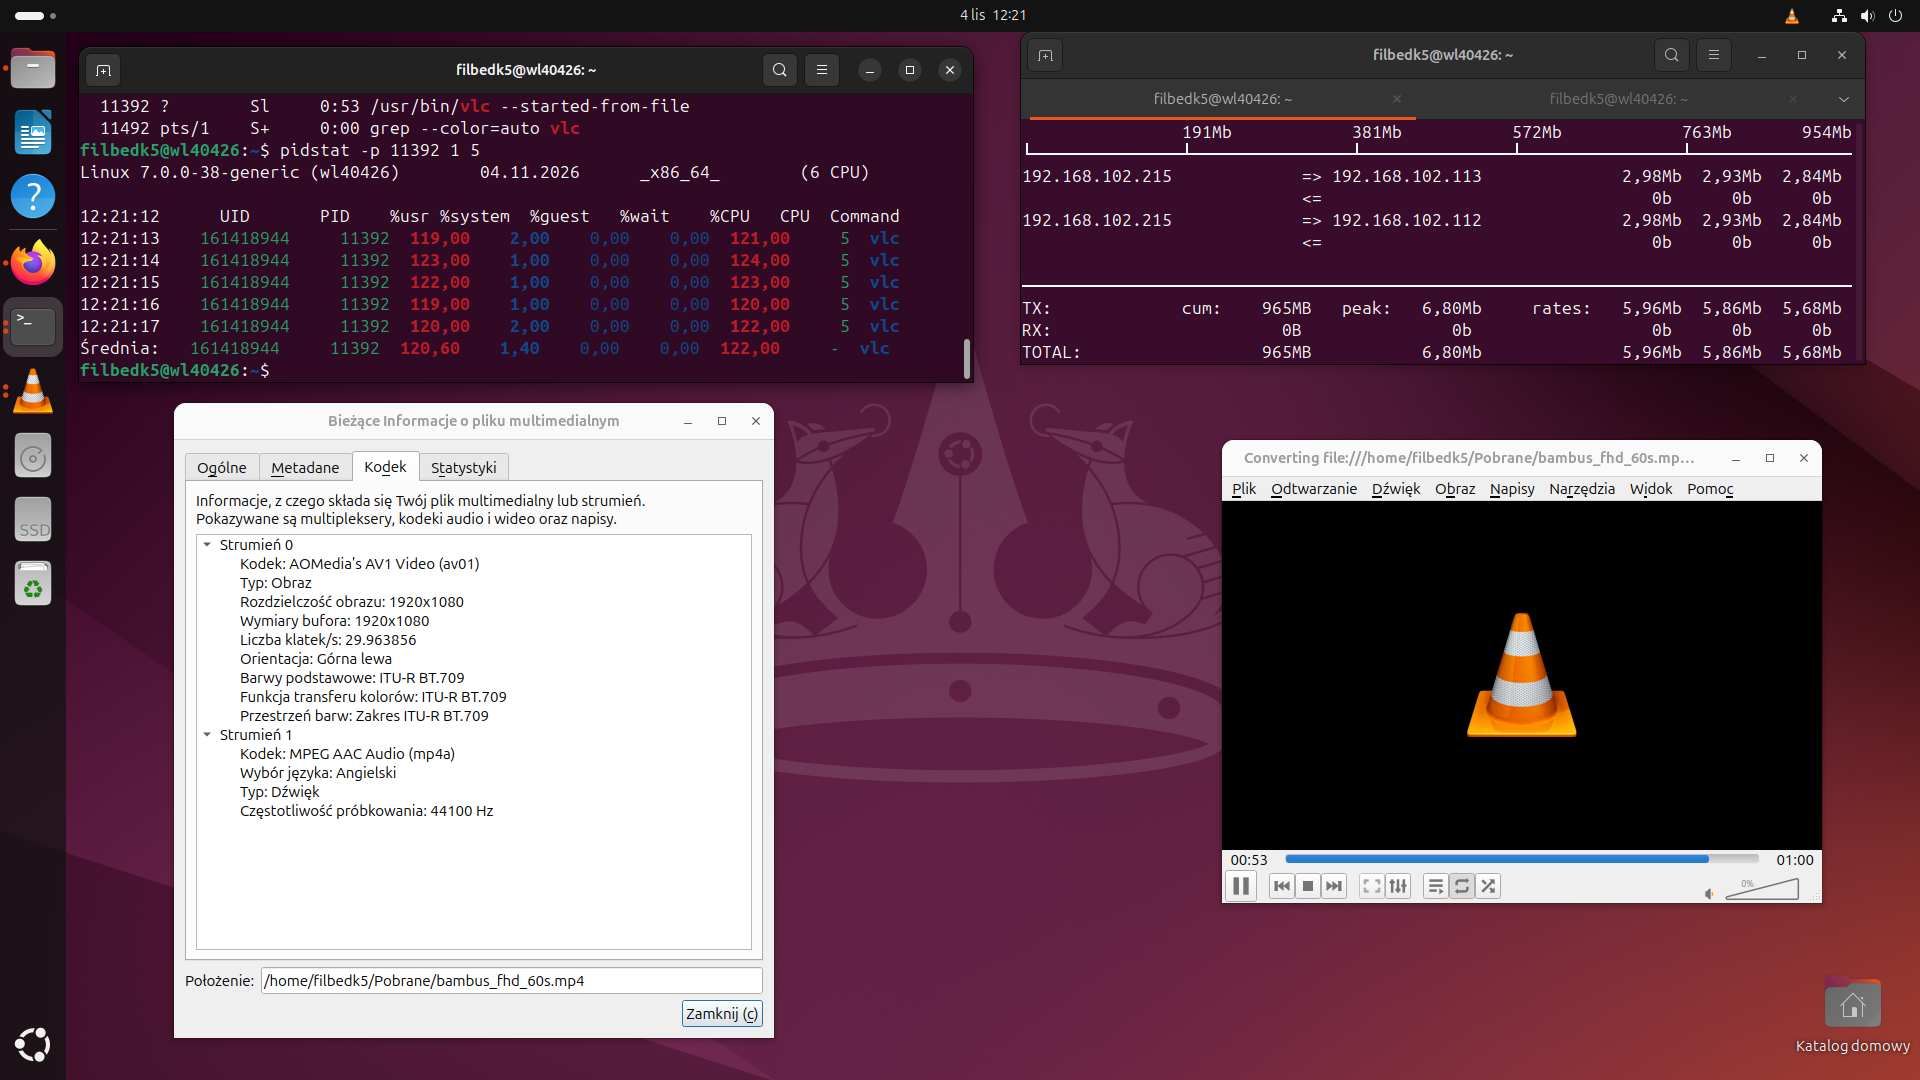
\includegraphics[width=\textwidth]{Zrzut ekranu z 2026-11-04 12-21-19.png}
        \caption{Serwer: Theora + Vorbis (FHD 1080p)}
    \end{subfigure}
    \hfill
    \begin{subfigure}[b]{0.48\textwidth}
        \centering
        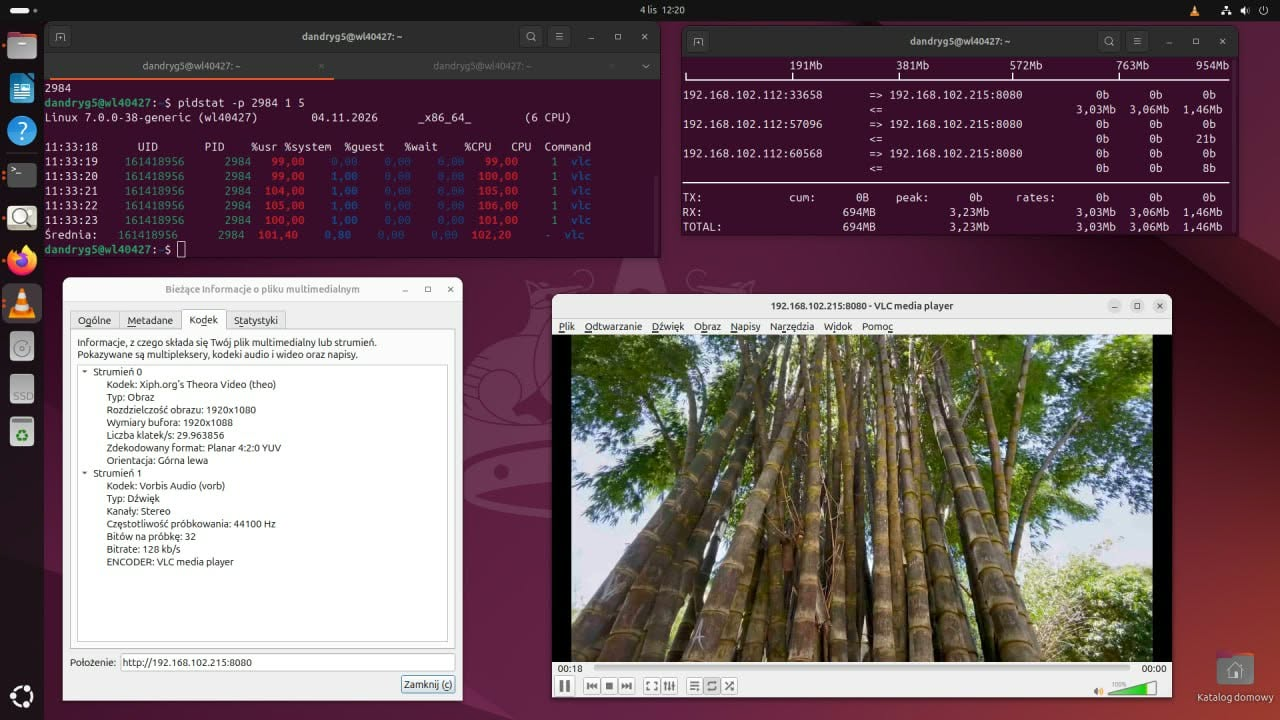
\includegraphics[width=\textwidth]{1000047920.jpg}
        \caption{Klient: Theora + Vorbis (FHD 1080p)}
    \end{subfigure}
    \caption{Pomiary dla profilu transkodowania Theora w rozdzielczości FHD.}
\end{figure}

% --- Test 9: Theora 2K ---
\begin{figure}[htbp]
    \centering
    \begin{subfigure}[b]{0.48\textwidth}
        \centering
        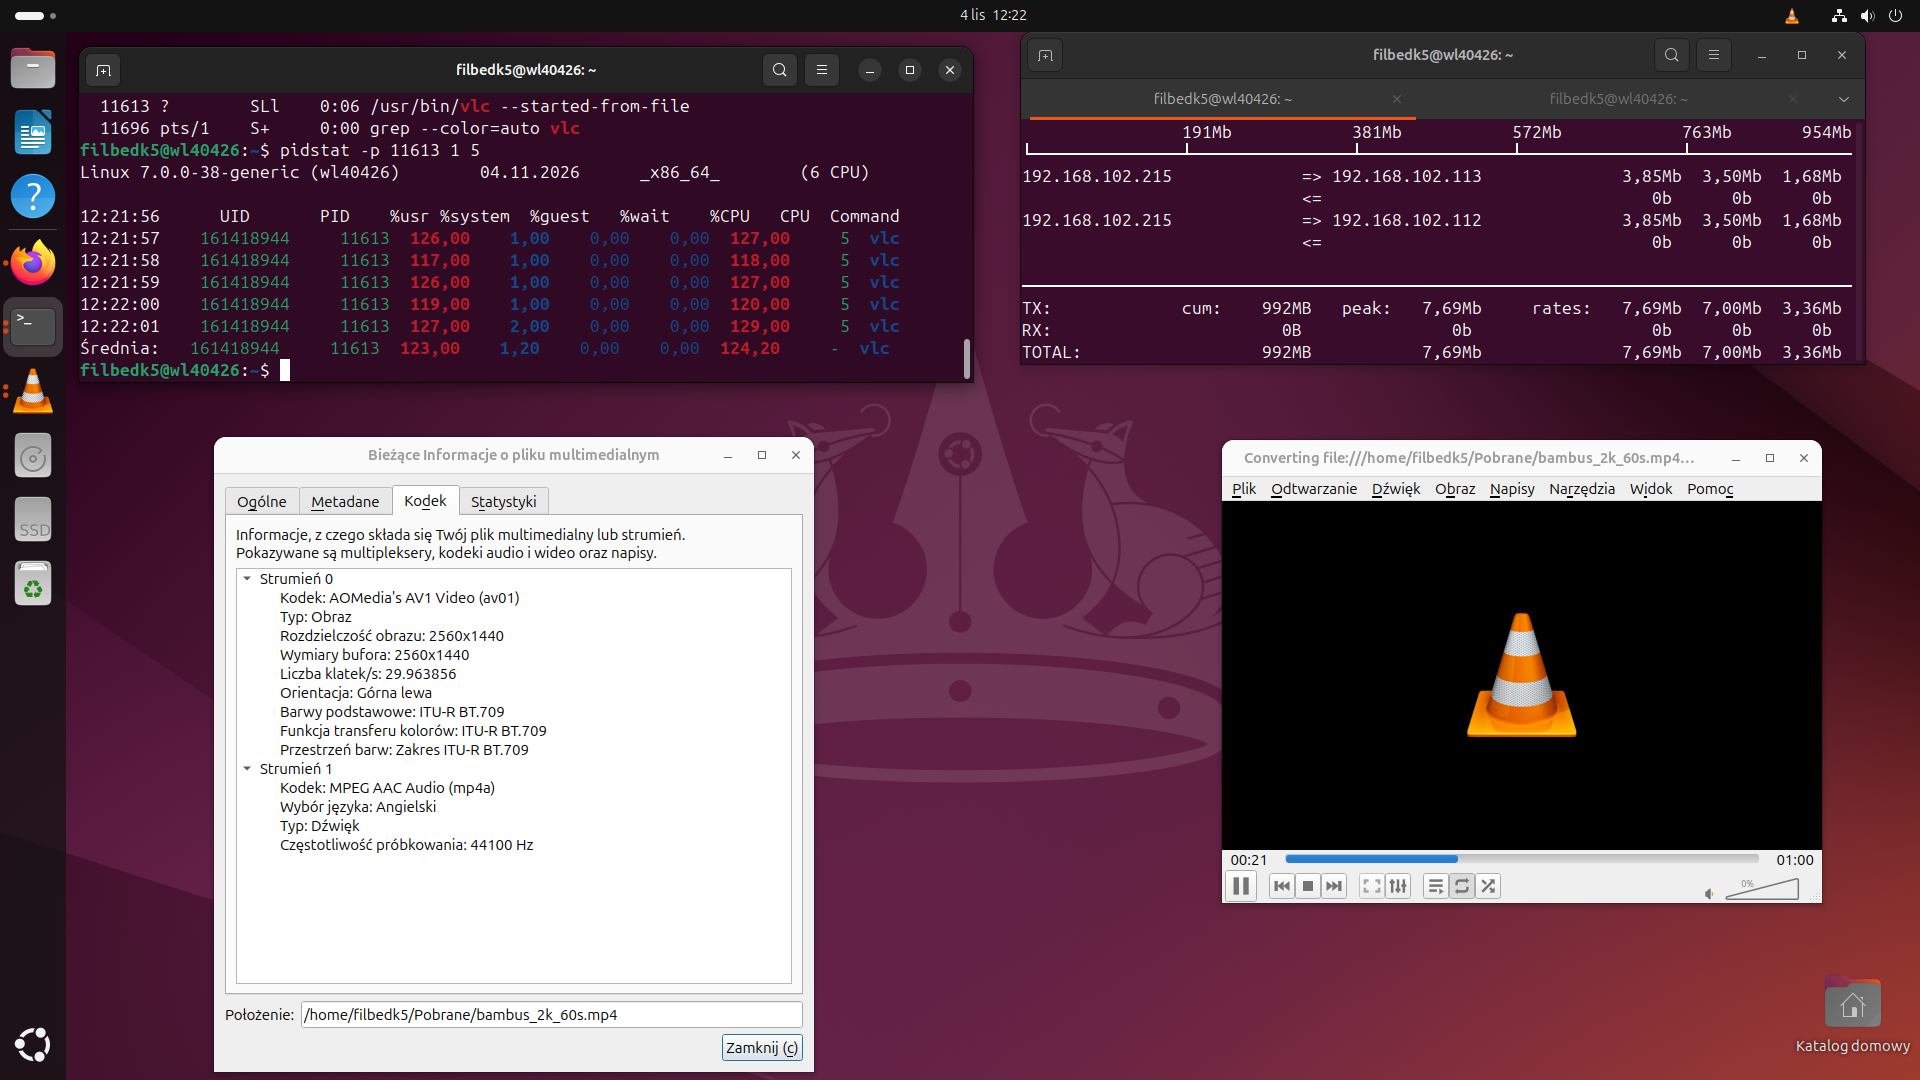
\includegraphics[width=\textwidth]{Zrzut ekranu z 2026-11-04 12-22-10.png}
        \caption{Serwer: Theora + Vorbis (2K/4K 1440p)}
    \end{subfigure}
    \hfill
    \begin{subfigure}[b]{0.48\textwidth}
        \centering
        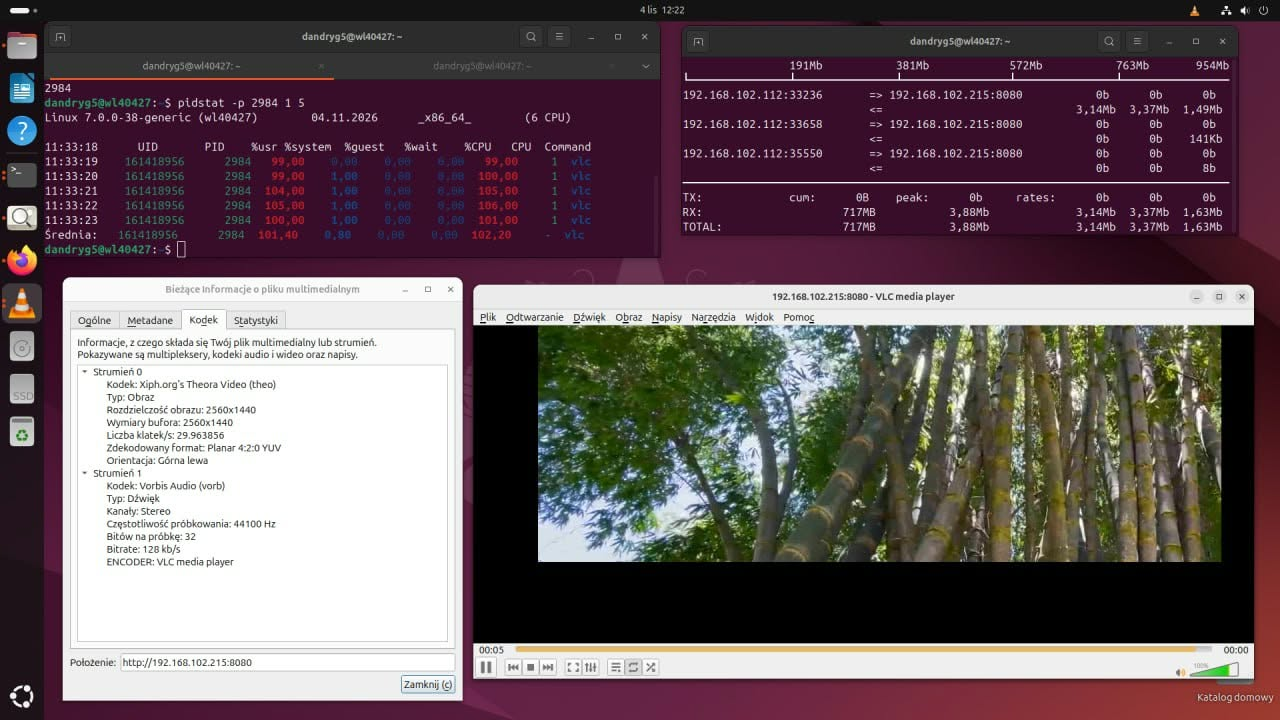
\includegraphics[width=\textwidth]{1000047926.jpg}
        \caption{Klient: Theora + Vorbis (2K/4K 1440p)}
    \end{subfigure}
    \caption{Pomiary dla profilu transkodowania Theora w rozdzielczości 2K/4K.}
\end{figure}

\clearpage


\section{Opracowanie wyników}

Na podstawie odczytanych danych poddaliśmy analizie wpływ parametrów kompresji na wydajność całego układu. 

\begin{itemize}
    \item \textbf{Wpływ kodeka na serwer (H.264 i H.265):} 
    Nowoczesny standard H.265 pozwalał na wyraźne zredukowanie ilości transmitowanych megabitów, natomiast okupione to było drastycznym wzrostem zasobożerności dla serwera w momencie konwersji plików (aż 589,40\% wykorzystania CPU dla wariantu 2K w H.265). Format H.264 pozostawał najbardziej przewidywalny – obciążenie procesora rosło proporcjonalnie do rozdzielczości.
    
    \item \textbf{Wydajność kodeka Theora:} 
    Kodek Theora we wszystkich testach osiągał słabe parametry (najniższy bitrate i wyjątkowo "niskie" zużycie CPU na poziomie 124\% dla wideo 2K). Ponieważ jest to przestarzały format, przypuszczamy, że enkoder zaimplementowany w odtwarzaczu operował w większości tylko na jednym rdzeniu, przez co nie nadążał kompresować pliku i masowo pomijał klatki. 

    \item \textbf{Obciążenie maszyny odbierającej:}
    Klient w niemal każdym teście zużywał ustaloną ilość zasobów procesora oscylującą w okolicy $102,20\%$. Oznacza to, że proces ciągłego dekodowania pakietów sieciowych z obojętnie jakiego zbadanych formatów wykorzystywał po stronie klienta pracę zbliżoną do maksymalnych możliwości wyłącznie jednego wątku/rdzenia.
\end{itemize}


\section{Wnioski}

\subsection{Wnioski szczegółowe}
\begin{enumerate}
    \item Kodek \textbf{H.265 (HEVC)} dostarczył bardzo dobre parametry, jeśli chodzi o oszczędność pasma przesyłowego (szczególnie widać to w plikach FHD i 2K, gdzie użył niemal połowę transferu niezbędnego dla H.264). Konsekwencją zastosowania tej kompresji jest jednak niezwykle intensywne obciążenie cpu po stronie nadającej strumień.
    \item Zestawiając wszystkie odczyty, dowiedliśmy, że standard \textbf{H.264} pozwalał zachować optymalny złoty środek – gwarantował płynny, nieprzerywany obraz i optymalne zużycie cpu.
    \item Wyniki strumieniowania w starym kodeku \textbf{Theora} były bardzo słabe. Niezdolność do optymalnej wielowątkowości sprawiła, że klatki były transmitowane niezwykle rzadko, a serwer nie był w stanie przetworzyć obrazu 2K w czasie rzeczywistym (wykorzystał do tego celu ok. 1.25 rdzenia).
\end{enumerate}

\subsection{Wnioski ogólne}
Przeprowadzone laboratorium wyraźnie zilustrowało kluczową rolę hardware'u w systemach live-streaming. Zauważyliśmy, że oszczędzanie zasobów infrastruktury sieciowej zawsze niesie ze sobą koszt w postaci znacznego dociążenia procesorów stacji nadawczych. Do popularnych streamów na żywo, o ile serwer nie jest wyposażony w dedykowany sprzętowy hardware encoding, wariantem bezkonkurencyjnym na podstawie naszych testów pozostaje kodek H.264.

\end{document}